
\section{Experiments} \label{sec:exp}

A prototype\footnote{Source code available at \url{https://github.com/jgorzny/Skeptik}} of a (two-traversal) version of {\SFOLowerUnits} has been implemented in the functional programming language Scala\footnote{\url{http://www.scala-lang.org/}} as part of the \skeptik
 library\footnote{\url{https://github.com/Paradoxika/Skeptik}}. 

Before evaluating this algorithm, we first generated several benchmark proofs. This was done by executing the {\SPASS}\footnote{\url{http://www.spass-prover.org/}} theorem prover on ToDo(numberOfProblems) problems of the ToDo categories of the TPTP Problem Library \footnote{\url{http://www.cs.miami.edu/{\textasciitilde}tptp/}}. In order to generate pure resolution proofs, most advanced inference rules used by {\SPASS}  were disabled. The Euler Cluster at the University of Victoria\footnote{\url{https://rcf.uvic.ca/euler.php}} was used and the time limit was 300 seconds per problem. Under these conditions, {\SPASS} was able to generate 308 proofs. 

The evaluation of {\SFOLowerUnits} was performed on a laptop (2.8GHz Intel Core i7 processor with 4 GB of RAM (1333MHz DDR3) available to the Java Virtual Machine). For each benchmark proof $\psi$, we measured\footnote{The raw data is available at ToDo (this link is not working) \url{https://docs.google.com/spreadsheets/d/1F1-t2OuhypmTQhLU6yTj42aiZ5CqqaZvhVvOzeFgn0k/edit\#gid=1182923972}} the time needed to compress the proof ($t(\psi)$) and the compression ratio ($(|\psi|-|\alpha(\psi)|)/|\psi|$), where $|\psi|$ is the length of $\psi$ (i.e. the number of axioms, resolution and contractions (ignoring substitutions)) and $\alpha(\psi)$ is the result of applying {\SFOLowerUnits} to $\psi$.

The proofs generated by {\SPASS} were small (with lengths from 3 to 49). These proofs are specially small in comparison with the typical proofs generated by SAT- and SMT-solvers, which usually have from a few hundred to a few million nodes. The number of proofs (compressed and uncompressed) per length is shown in Figure \ref{fig:ex} (b). Uncompressed proofs are those which had either no lowerable units to lower or for which \SFOLowerUnits failed and returned the original proof. Such failures occurred on only 14 benchmark proofs. Among the smallest of the 308 proofs, very few proofs were compressed. This is to be expected, since the likelihood that a very short proof contain a lowerable unit (or even merely a unit with more than one child) is low. The proportion of compressed proofs among longer proofs is, as expected, larger, since they have more nodes and it is more likely that some of these nodes are lowerable units. 13 out of 18 proofs with length greater than or equal to 30 were compressed. 

Figure \ref{fig:ex} (a) shows a box-whisker plot of compression ratio with proofs grouped by length and whiskers indicating minimum and maximum compression ratio achieved within the group. Besides the median compression ratio (the horizontal thick black line), the chart also shows the mean compression ratios for all proofs of that length and for all compressed proofs (the red cross and the blue circle). In the longer proofs (length greater than 34), the median and the means are in the range from 5\% to 15\%, which is satisfactory in comparison with the total compression ratio of 7.5\% that has been measured for the propositional {\LowerUnits} algorithm on much longer propositional proofs \cite{Boudou}.

Figure \ref{fig:ex} (c) shows a scatter plot comparing the length of the input proof against the length of the compressed proof. For the longer proofs (circles in the right half of the plot), it is often the case that the length of the compressed proof is significantly lesser than the length of the input proof.

Figure \ref{fig:ex} (d) plots the cumulative original and compressed lengths of all benchmark proofs (for an x-axis value of $k$, the cumulative curves show the sum of the lengths of the shortest $k$input proofs). The total cumulative length of all original proofs is ToDo:4500(put the correct number here) while the cumulative length of all proofs after compression is ToDo:4000(correct this number). This results in a total compression ratio of ToDo:12\%(compute this number), which is impressive, considering the inclusion of all the short proofs (in which the presence of lowerable units is a priori unlikely) tends to decrease the total compression ratio. For comparison, the total compression ratio considering only the 100 longest input proofs is ToDo:(compute this percentage).

Figure \ref{fig:ex} also indicates an interesting potential trend. The gap between the two cumulative curves seems to grow superlinearly. If this trend is extrapolated, progressively larger compression ratios can be expected for longer proofs. This is compatible with Theorem 10 in \cite{RPILU}, which shows that, for proofs generated by eagerly resolving units against all clauses, the propositional {\LowerUnits} algorithm can achieve quadratic assymptotic compression. SAT- and SMT-solvers based on CDCL (Conflict-Driven Clause Learning) avoid eagerly resolving unit clauses by dealing with unit clauses via boolean propagation on a conflict graph and extracting subproofs from the conflict graph with every unit being used at most once per subproof (even when it was used multiple times in the conflict graph). Saturation-based automated theorem provers, on the other hand, might be susceptible to the eager unit resolution redundancy described in Theorem 10 \cite{RPILU}. This potential trend would need to be confirmed by further experiments with more data (more proofs and longer proofs).

The total time needed by {\SPASS} to generate all 308 proofs on the Euler Cluster was ToDo. The total time for {\SFOLowerUnits} to be executed on all 308 proofs was ToDo on a simple laptop. (ToDo: make sure the total time calculation either includes or excludes parsing times for both Skeptik and SPASS. otherwise the comparison would be biased and unfair). Therefore, {\SFOLowerUnits} is a fast algorithm. For a small overhead in time (in comparison to proving time), it may simplify the proof considerably.


% \begin{figure}
% 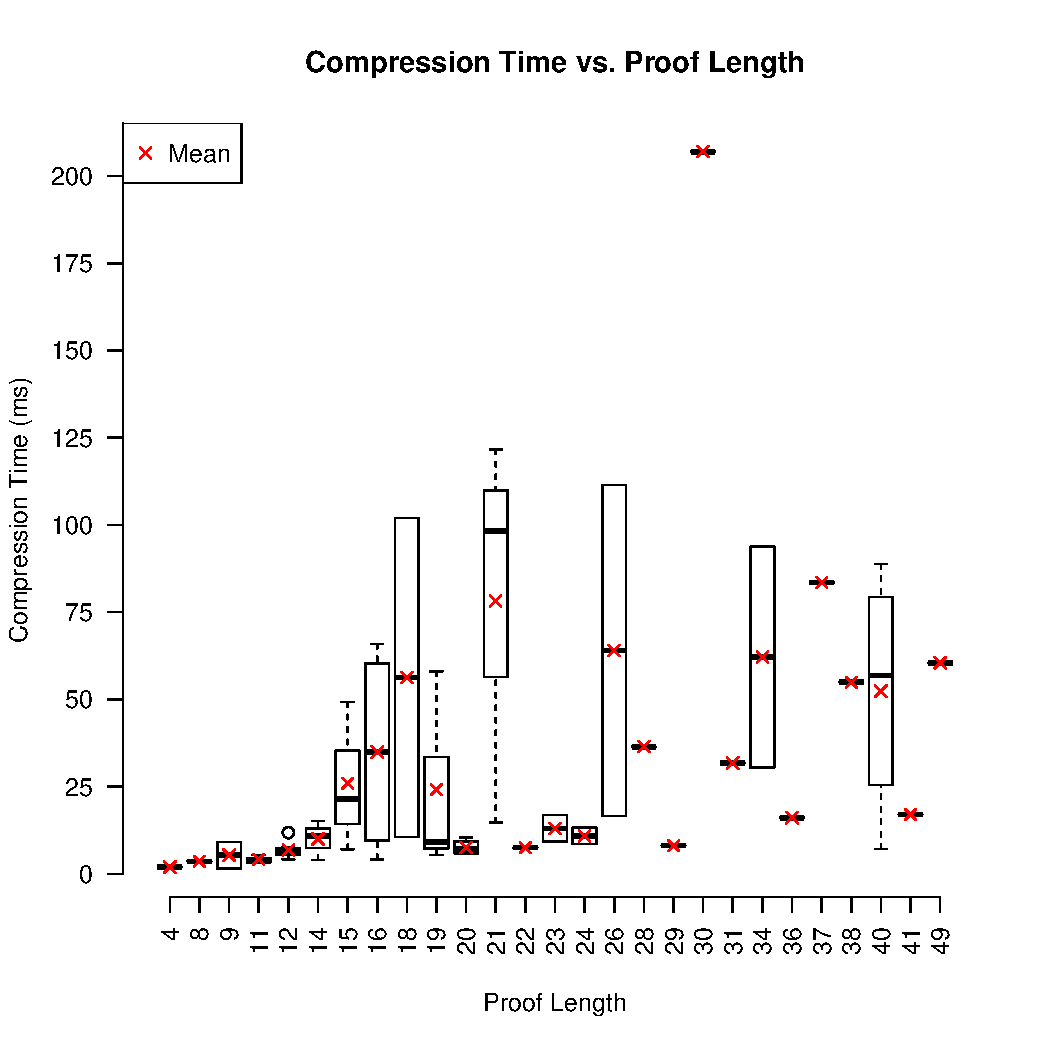
\includegraphics[scale=0.5]{images/compress_time_vs_proof_length.pdf}
% \end{figure}

% \begin{figure}
% 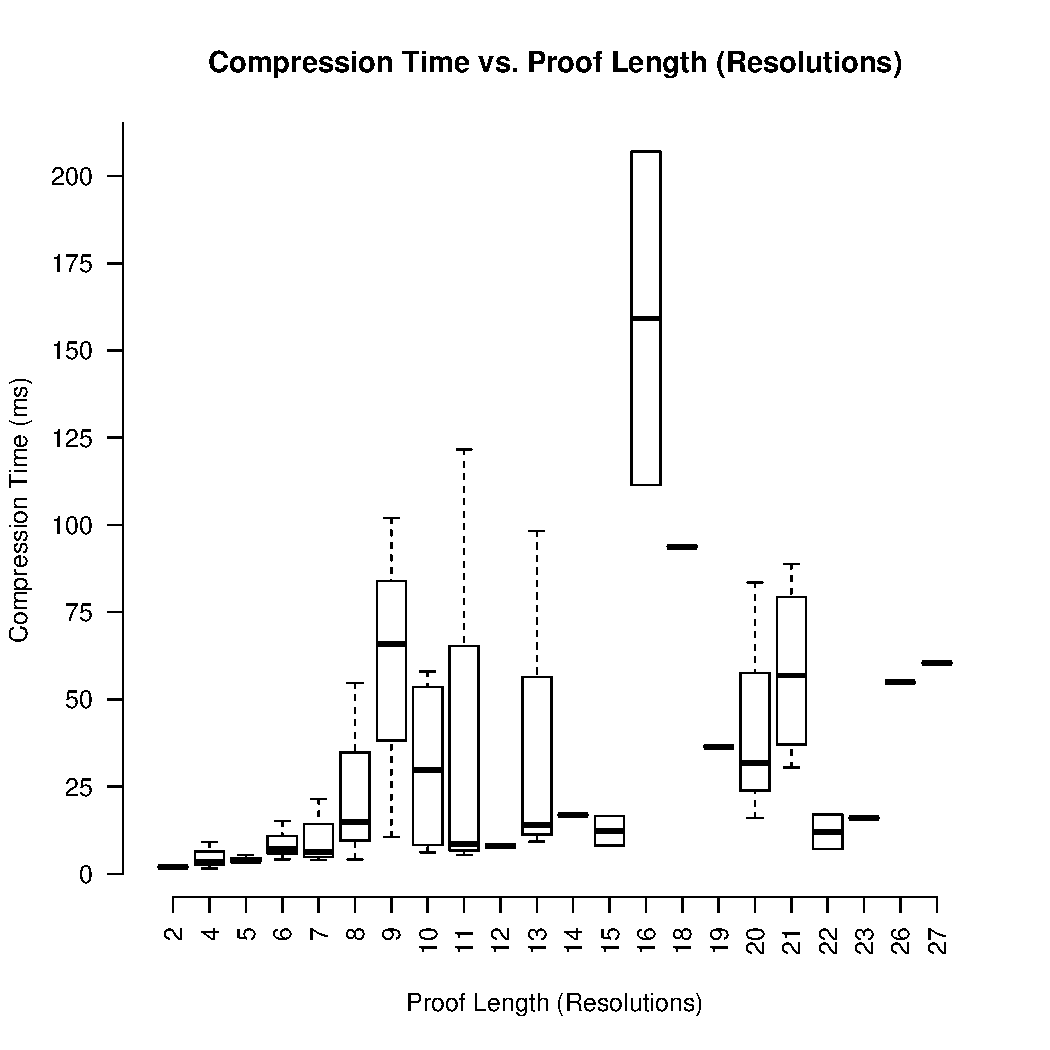
\includegraphics[scale=0.5]{images/compress_time_vs_proof_length_res.pdf}
% \end{figure}

% \begin{figure}
% 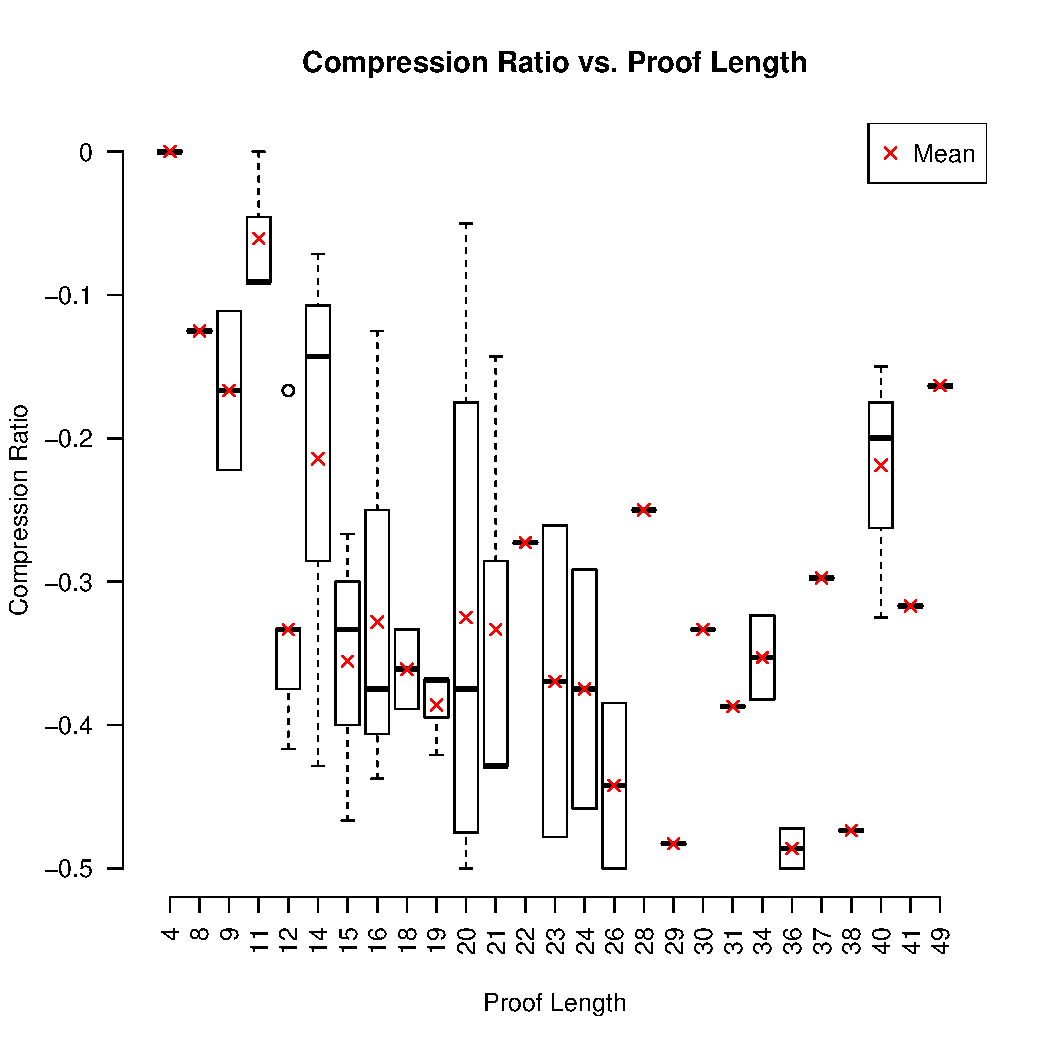
\includegraphics[scale=0.5]{images/compress_ratio_vs_proof_length.pdf}
% \end{figure}

%\begin{figure}\label{fig:compressRatioResVLength} %USED
%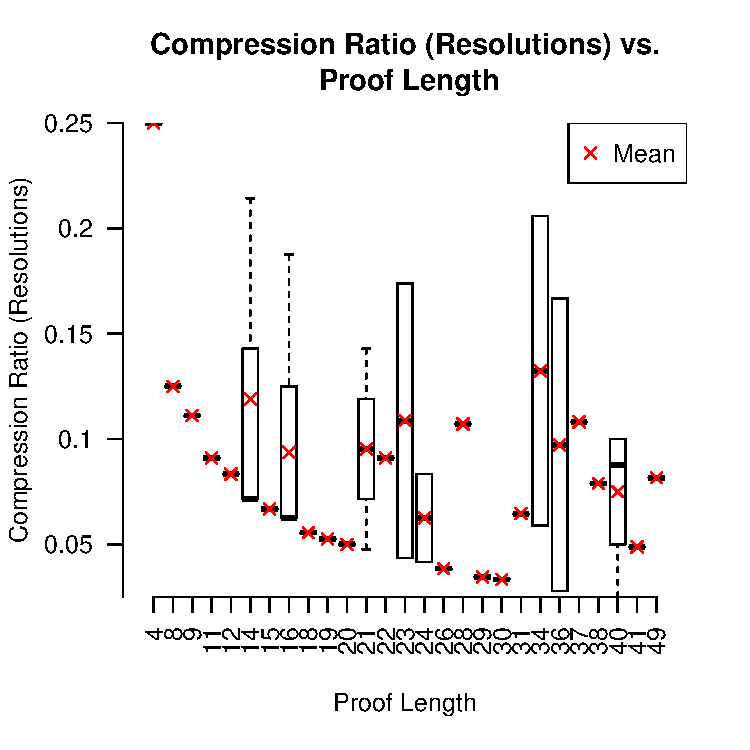
\includegraphics[scale=0.5]{images/compress_ratio_res_vs_proof_length.pdf}
%\end{figure}

% \begin{figure}
% 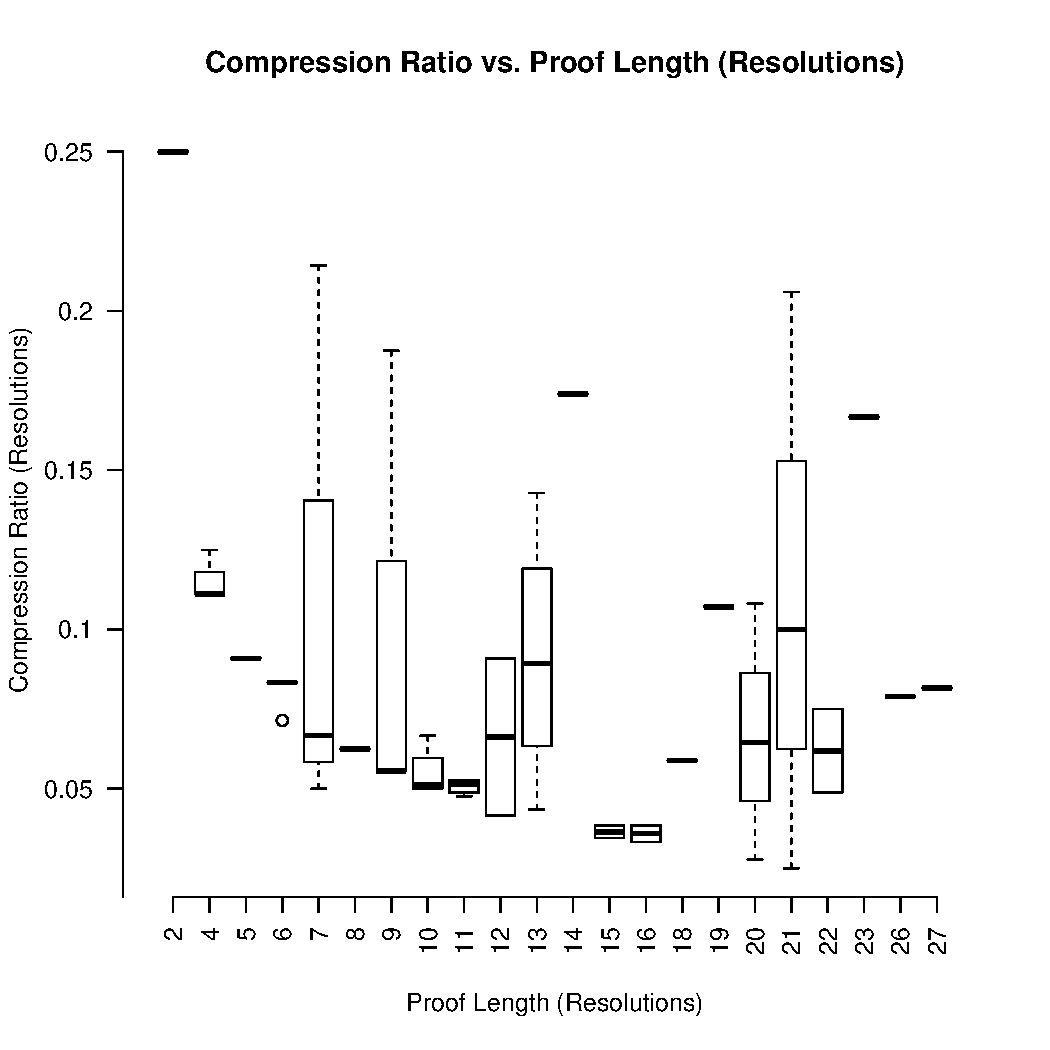
\includegraphics[scale=0.5]{images/compress_ratio_res_vs_proof_length_res.pdf}
% \end{figure}

%\begin{figure}%USED
%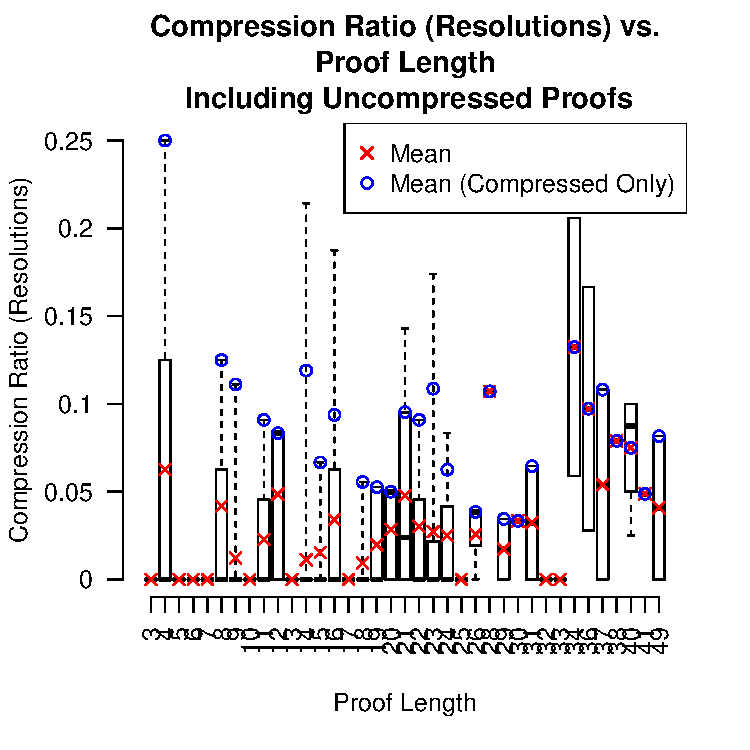
\includegraphics[scale=0.5]{images/compress_ratio_res_vs_proof_length_all_proofs.pdf}
%\end{figure}
\begin{figure}
\centering
%    \subfloat[Average compression (only success)]{{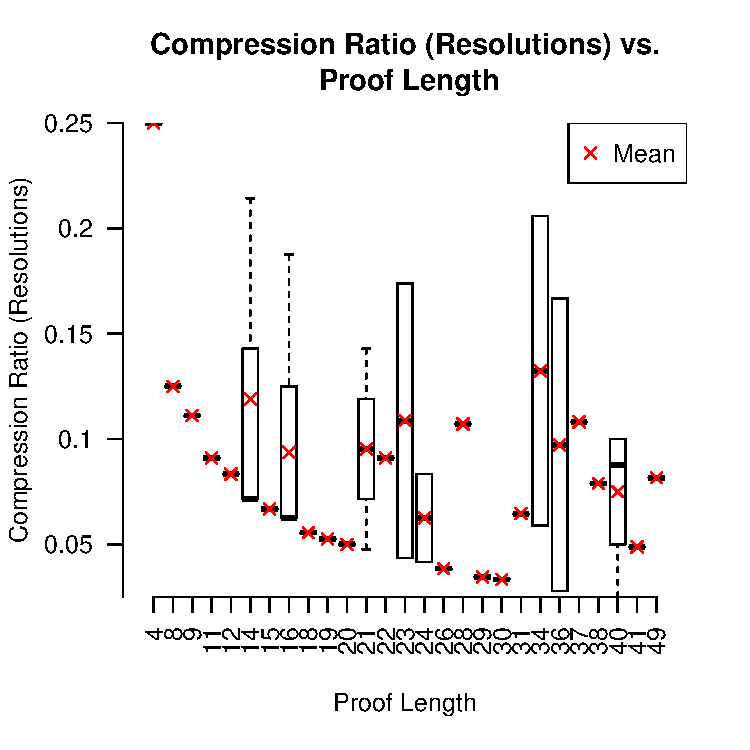
\includegraphics[scale=0.5]{images/compress_ratio_res_vs_proof_length.pdf} }}
    \subfloat[Overall average compression]{{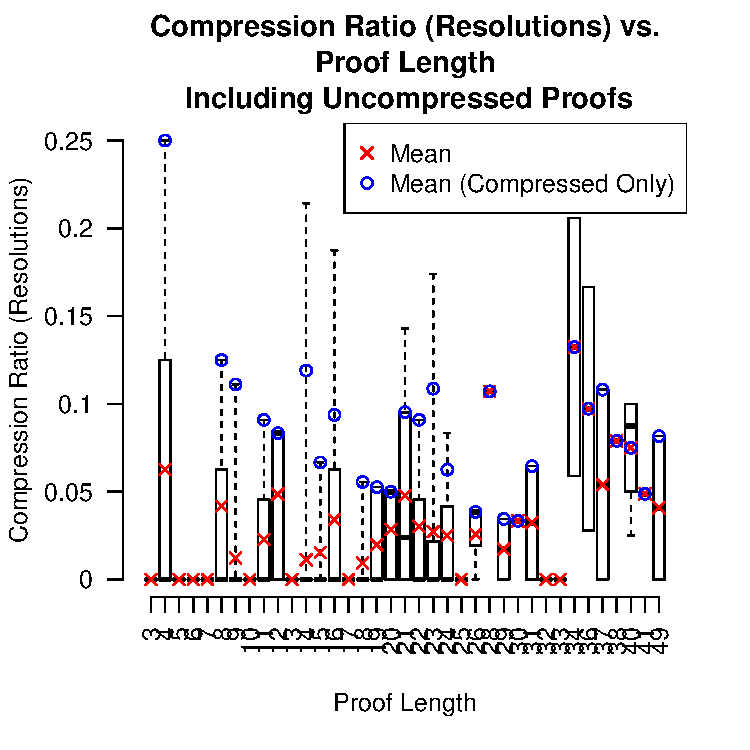
\includegraphics[scale=0.5]{images/compress_ratio_res_vs_proof_length_all_proofs.pdf} }}%\hfilll
    \subfloat[Number of proofs of each length compressed]{{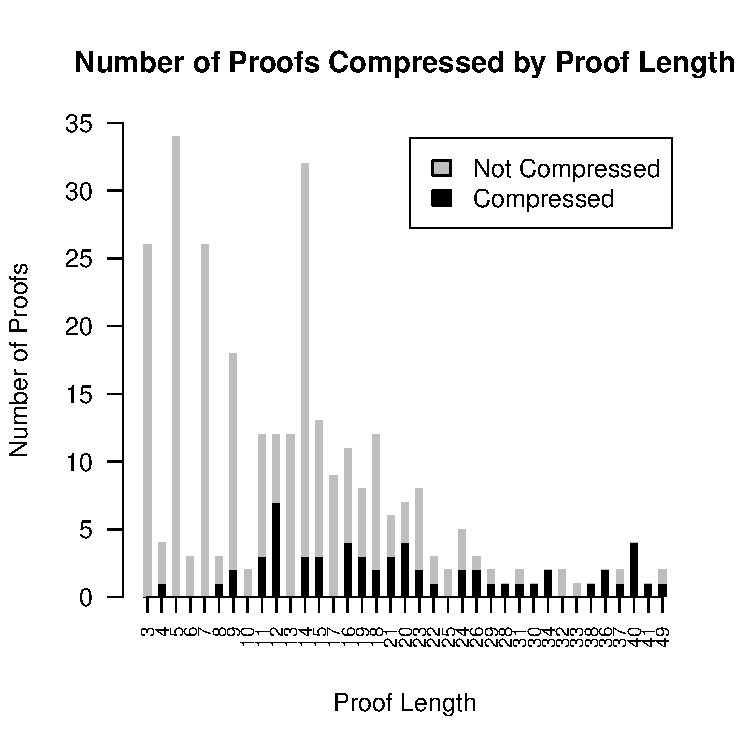
\includegraphics[scale=0.5]{images/num_compressed_stacked.pdf}}}\hfill
    \subfloat[Compressed length against input length]{{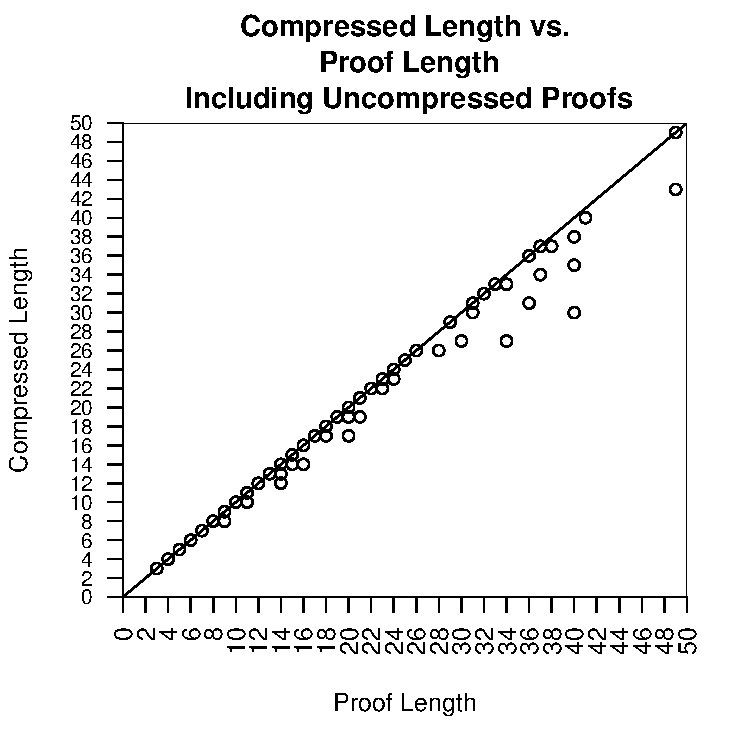
\includegraphics[scale=0.5]{images/compress_length_no_sub_vs_length_all_proofs.pdf} }}
%    \subfloat[Total proof nodes]{{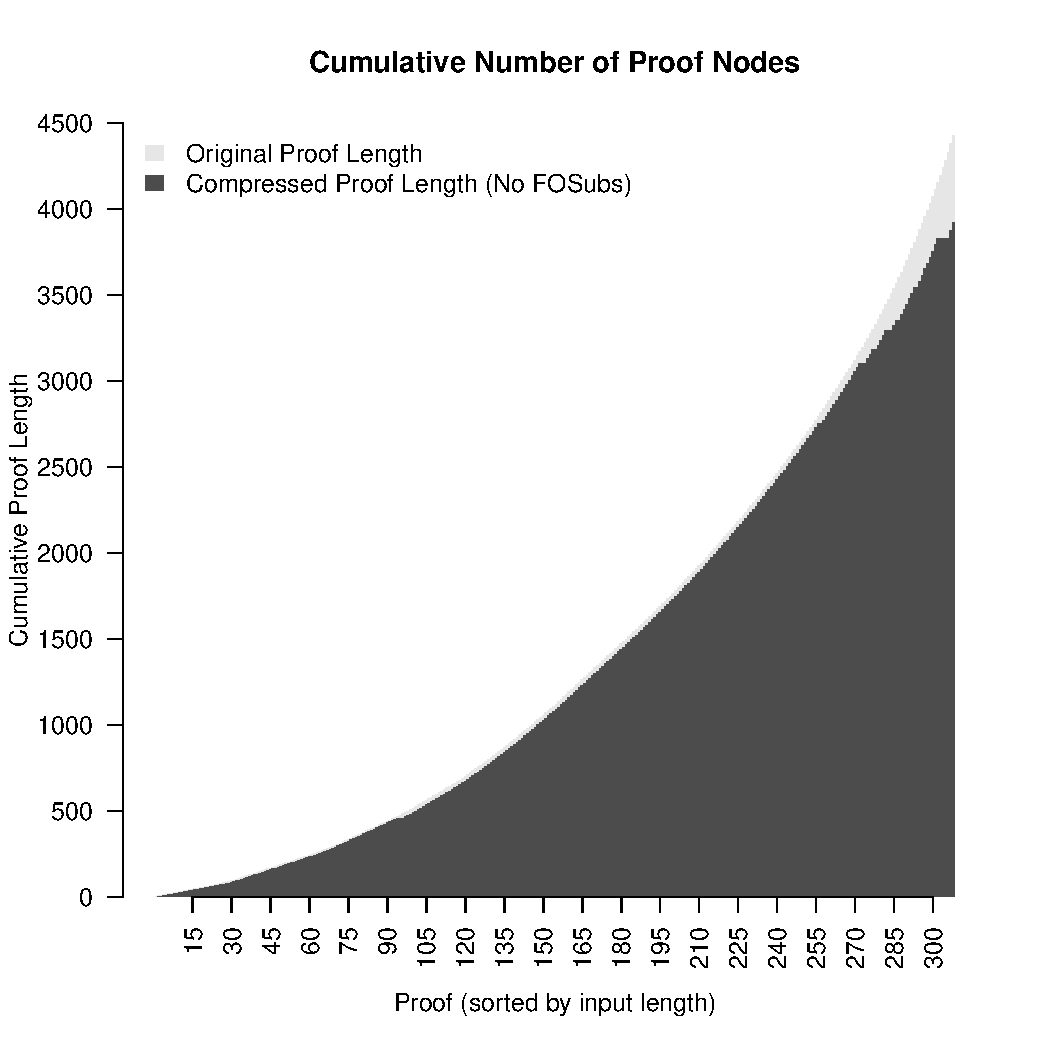
\includegraphics[scale=0.5]{images/cumulative_res_nodes_no_subs.pdf} }}
    \subfloat[Node reduction resulting from 100 largest proofs]{{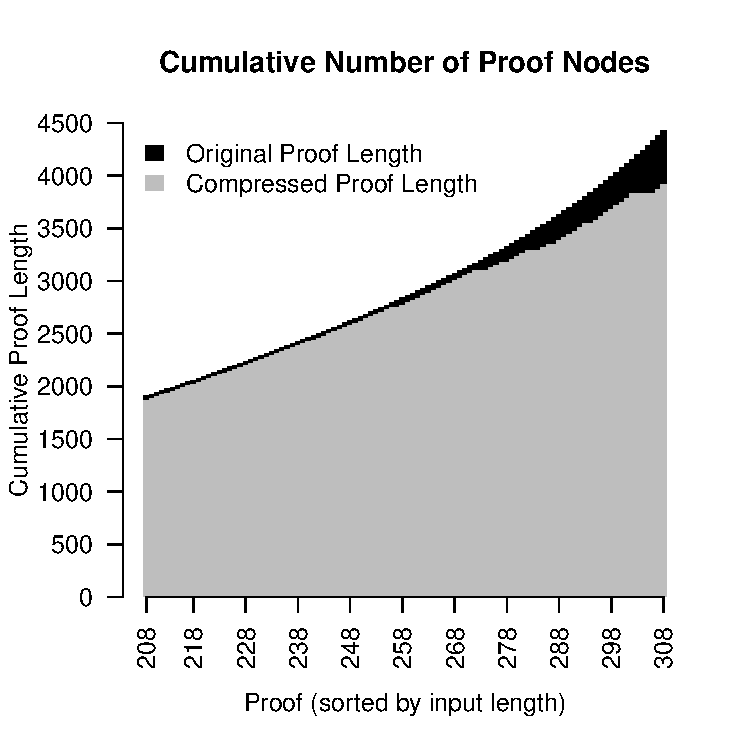
\includegraphics[scale=0.5]{images/cumulative_res_nodes_no_subs_top100.pdf}}}
\caption{Empirical evaluation results.}
\label{fig:ex}
\end{figure}


%\begin{figure}
%\centering
%    \subfloat{{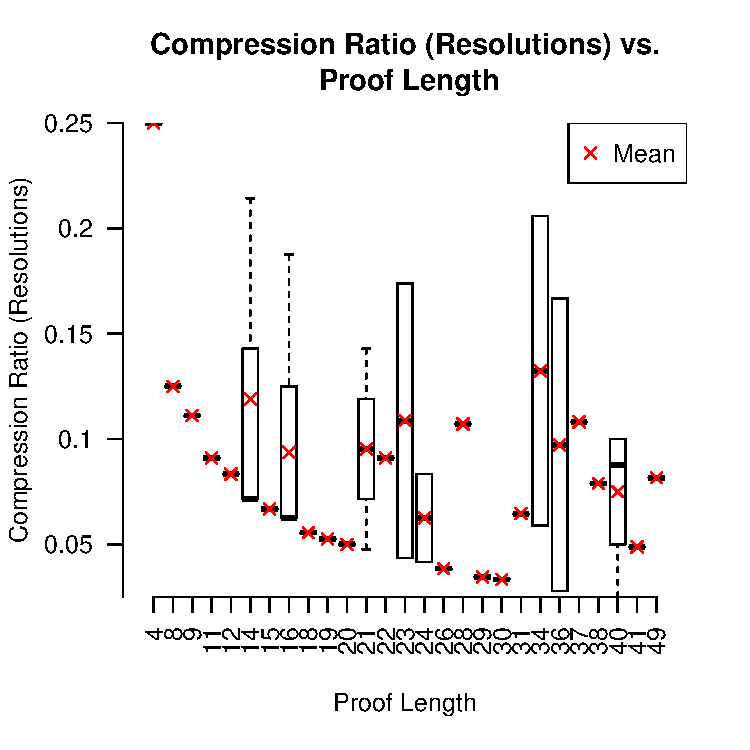
\includegraphics[scale=0.5]{images/compress_ratio_res_vs_proof_length.pdf}
%}}%
%    \subfloat{{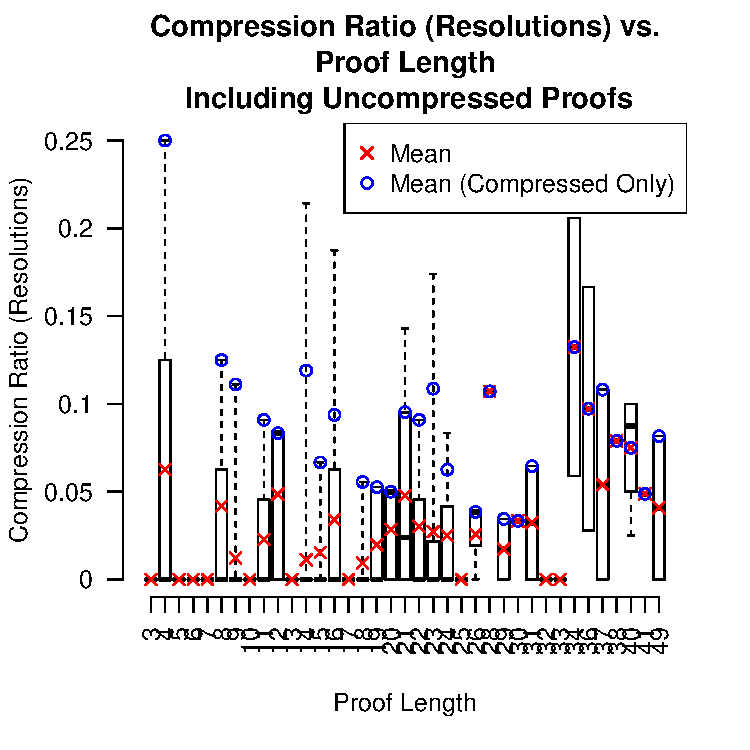
\includegraphics[scale=0.5]{images/compress_ratio_res_vs_proof_length_all_proofs.pdf} }}%
%\caption{Compression ratio versus proof length without uncompressed proofs (left) and with with uncompressed proofs (right).}
%\label{fig:ex1}
%\end{figure}



% \begin{figure}
% 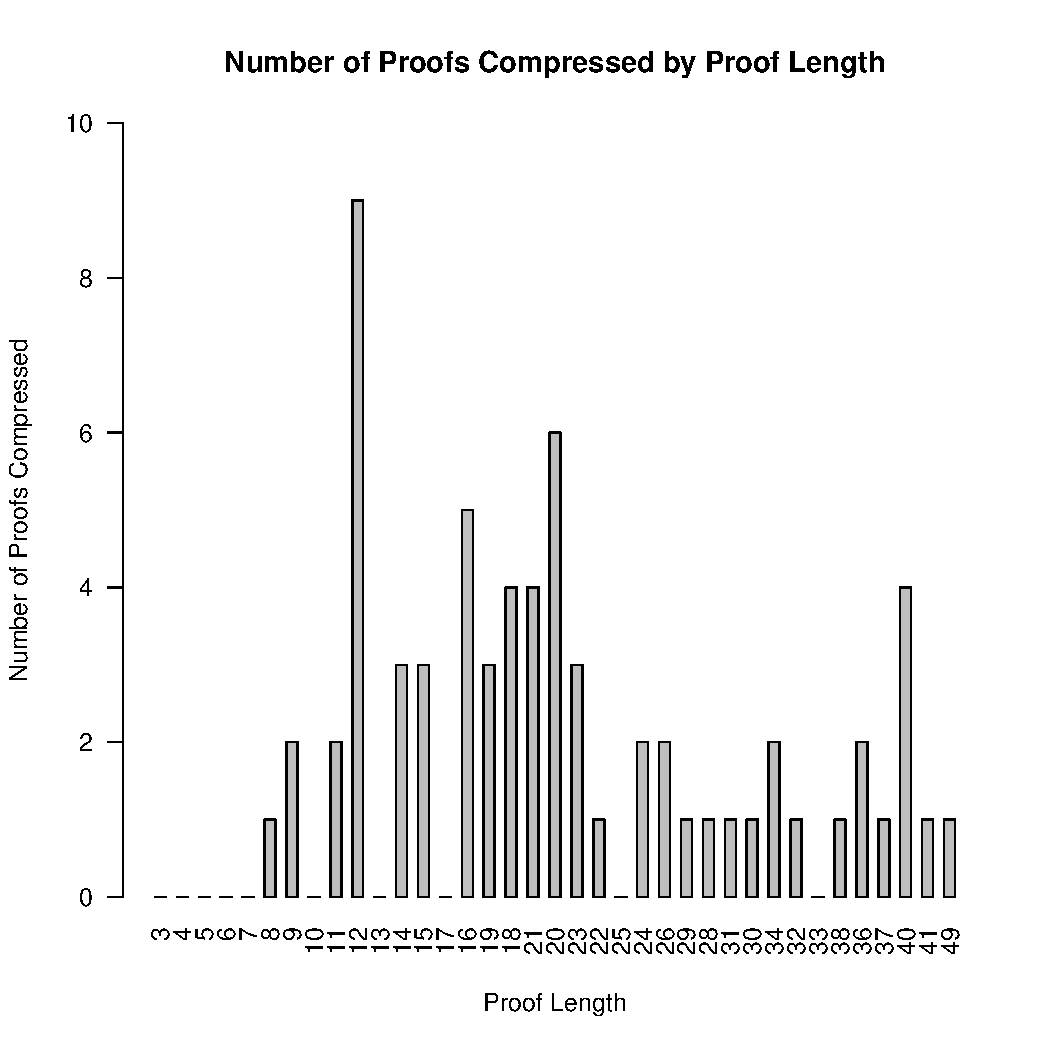
\includegraphics[scale=0.5]{images/num_compressed_count.pdf}
% \end{figure}

% \begin{figure}
% 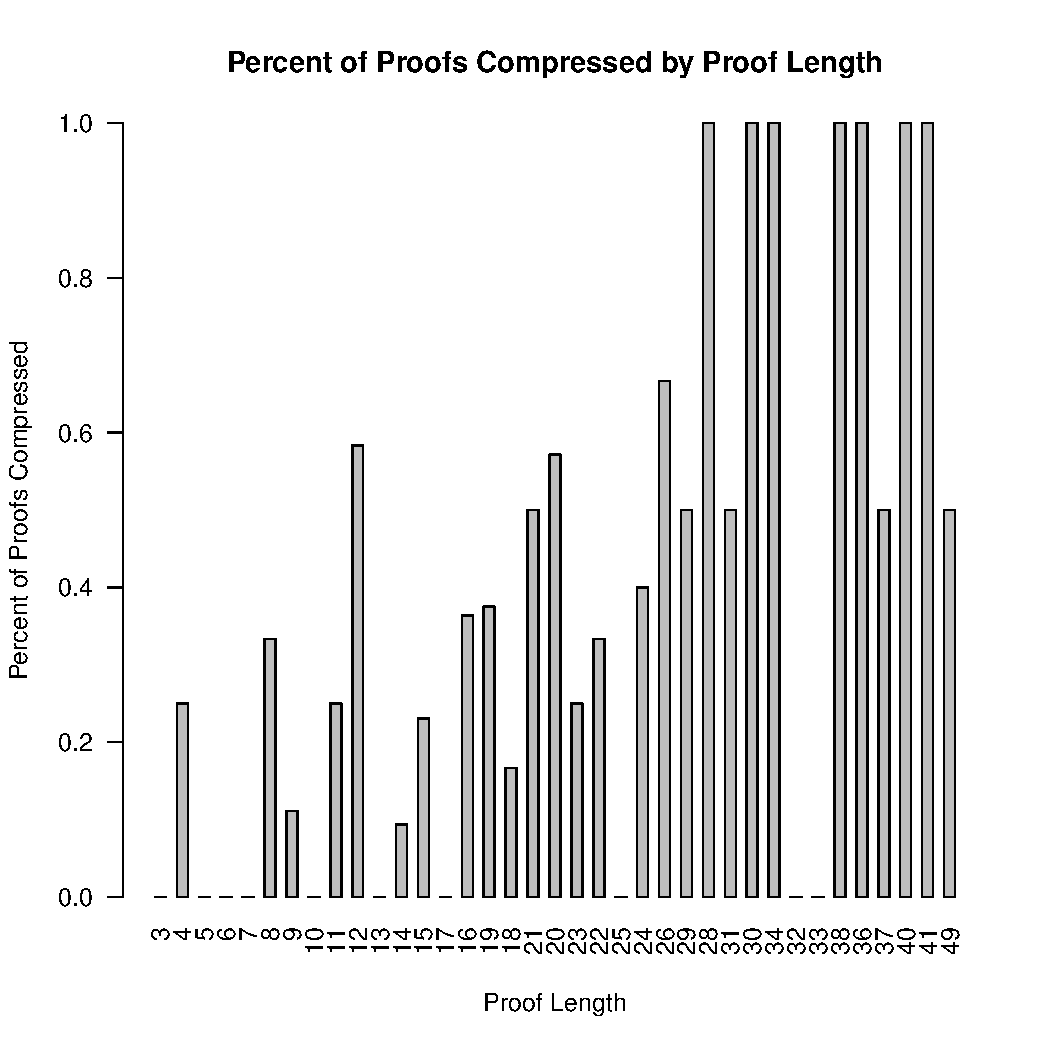
\includegraphics[scale=0.5]{images/num_compressed_percent.pdf}
% \end{figure}


%\begin{figure}%USED
%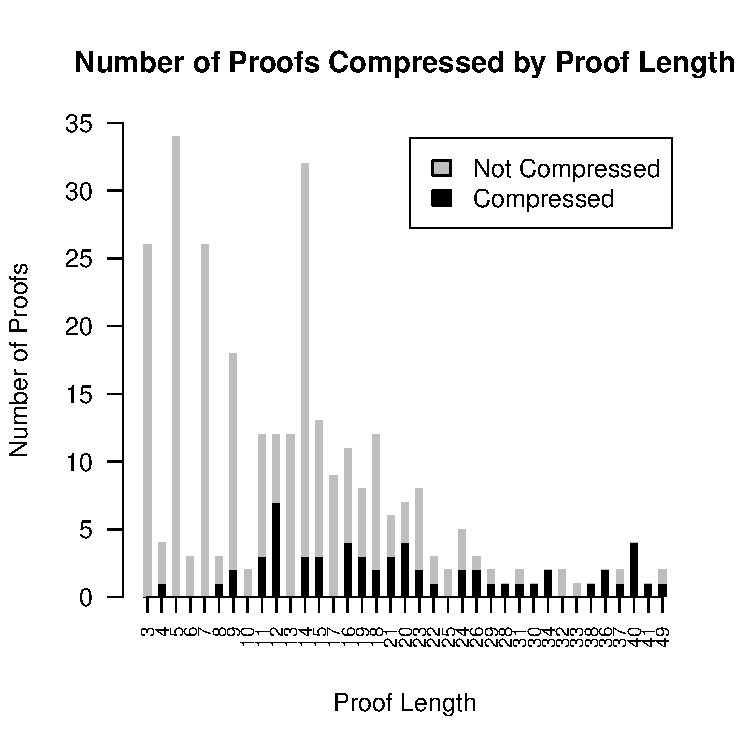
\includegraphics[scale=0.5]{images/num_compressed_stacked.pdf}
%\end{figure}

%\begin{figure}
%\centering
%    \subfloat{{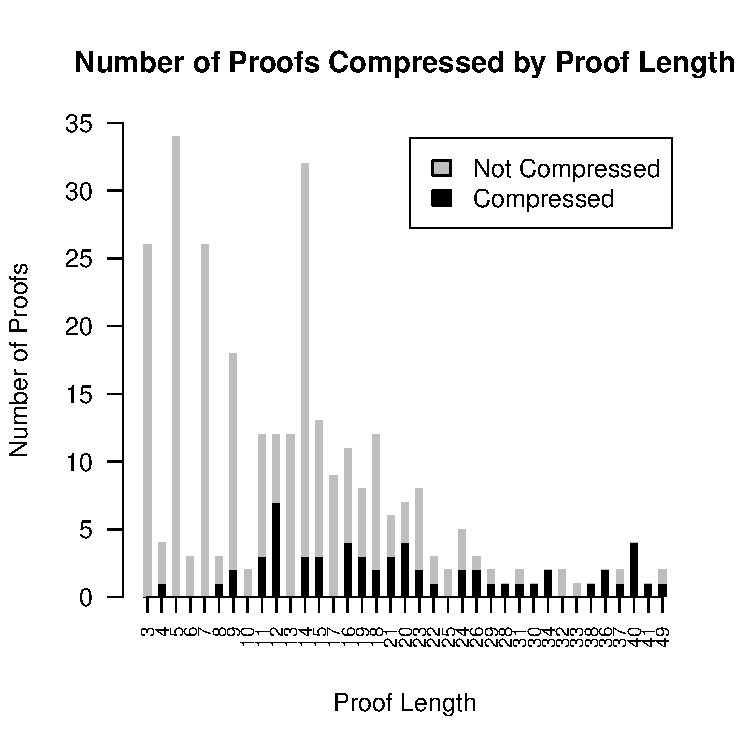
\includegraphics[scale=0.5]{images/num_compressed_stacked.pdf}
%}}%
%    \subfloat{{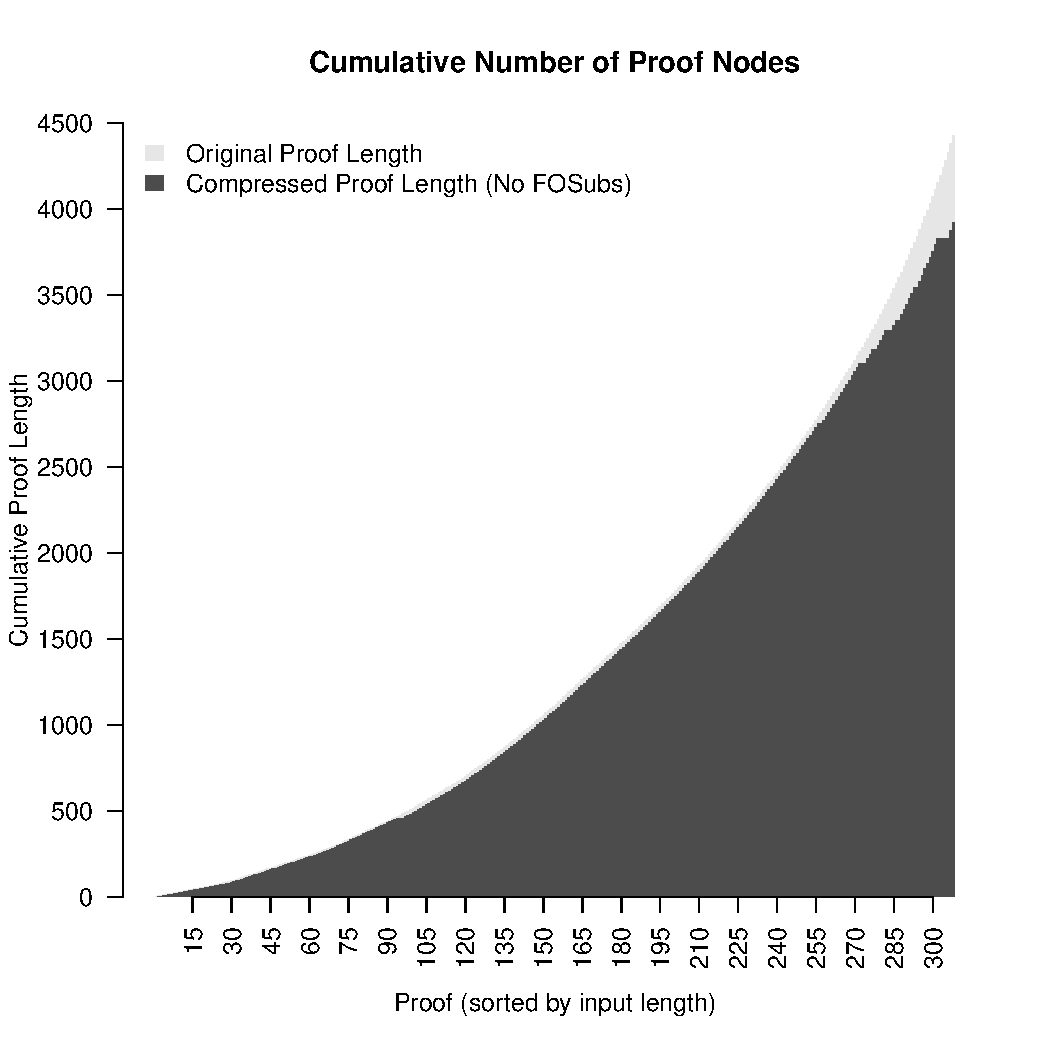
\includegraphics[scale=0.5]{images/cumulative_res_nodes_no_subs.pdf} }}
%\caption{Number of proofs compressed of each length (left), and total number of nodes before and after compression (right).}
%\label{fig:ex2}
%\end{figure}


% \begin{figure}
% 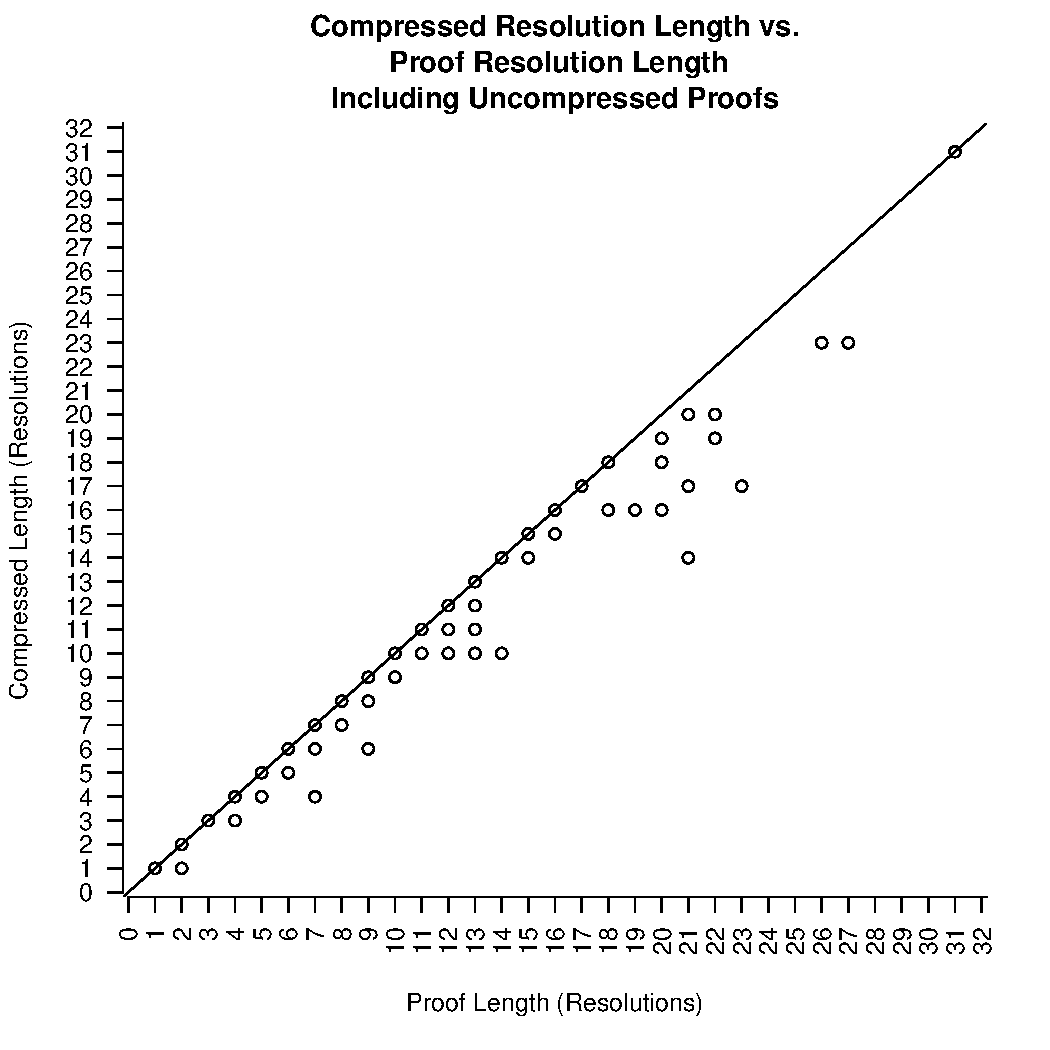
\includegraphics[scale=0.5]{images/res_length_vs_compress_res_length_all_proofs.pdf}
% \end{figure}
% \begin{figure}
% 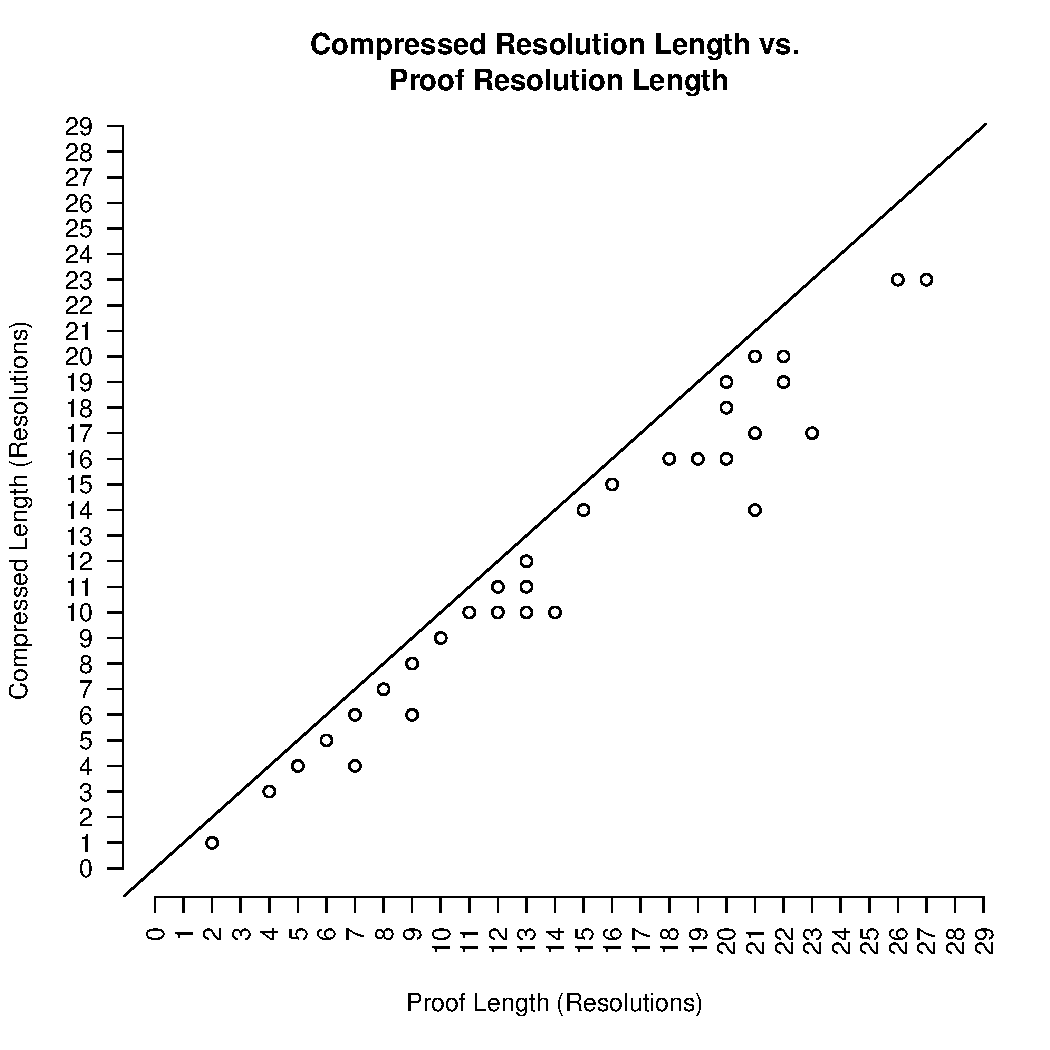
\includegraphics[scale=0.5]{images/res_length_vs_compress_res_length.pdf}
% \end{figure}

% \begin{figure}
% 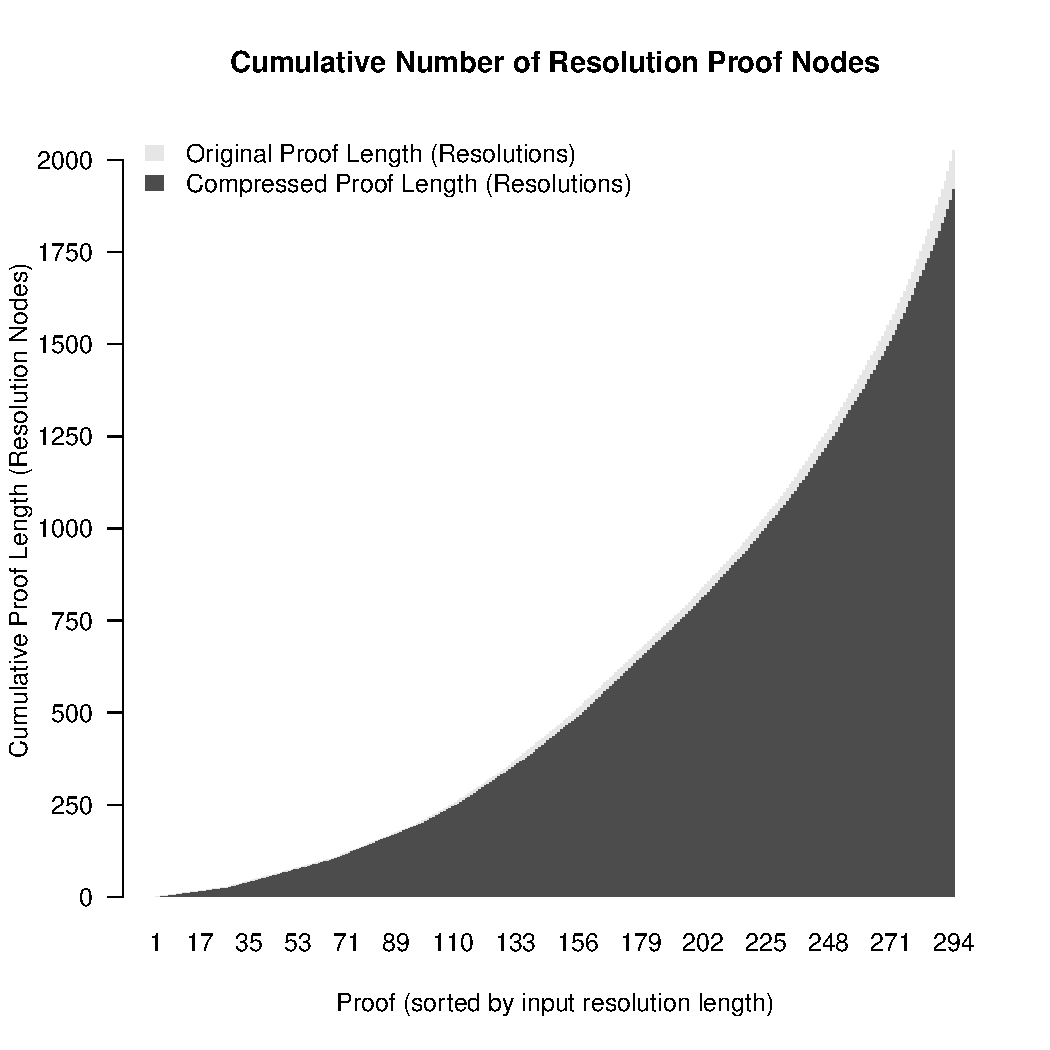
\includegraphics[scale=0.5]{images/cumulative_res_nodes.pdf}
% \end{figure}

%\begin{figure}%USED
%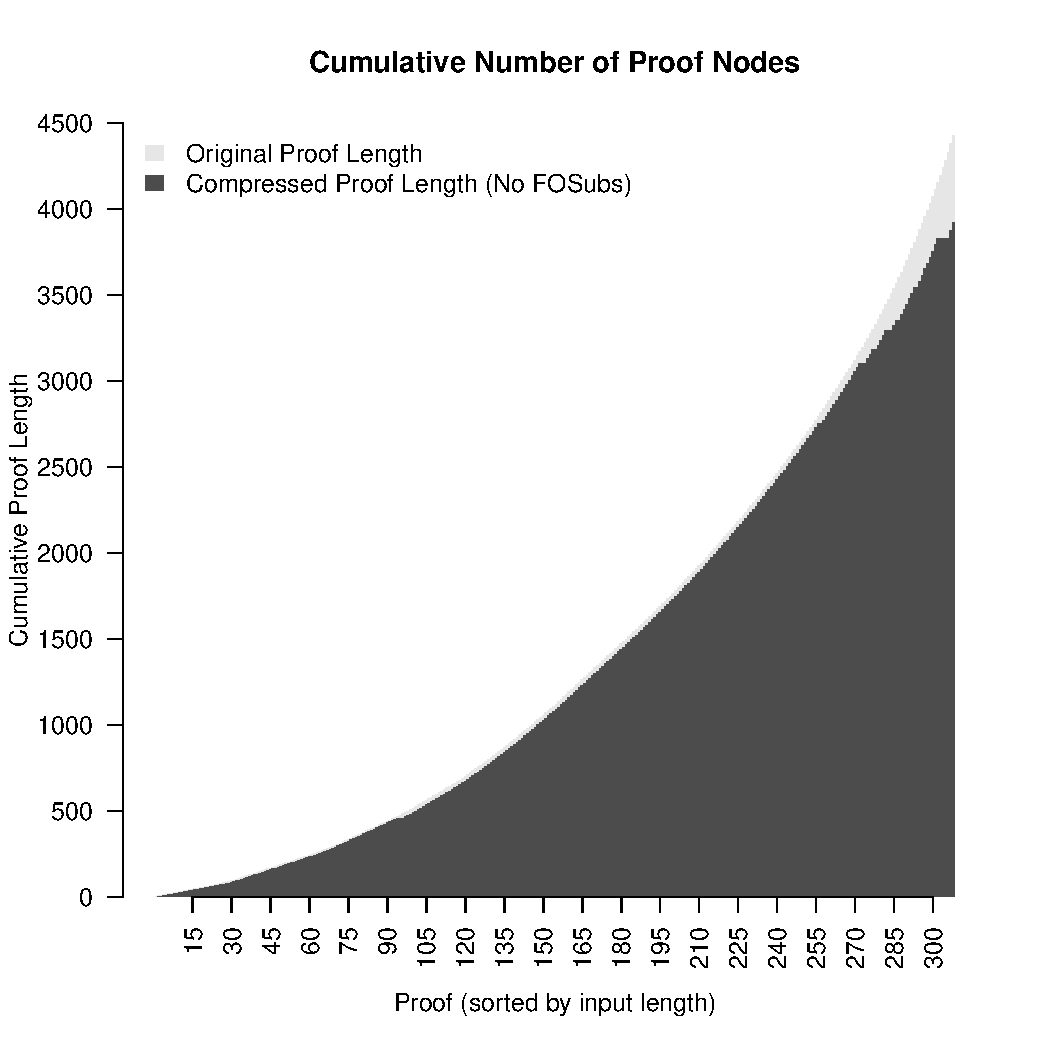
\includegraphics[scale=0.5]{images/cumulative_res_nodes_no_subs.pdf}
%\end{figure}

%\begin{figure} %USED
%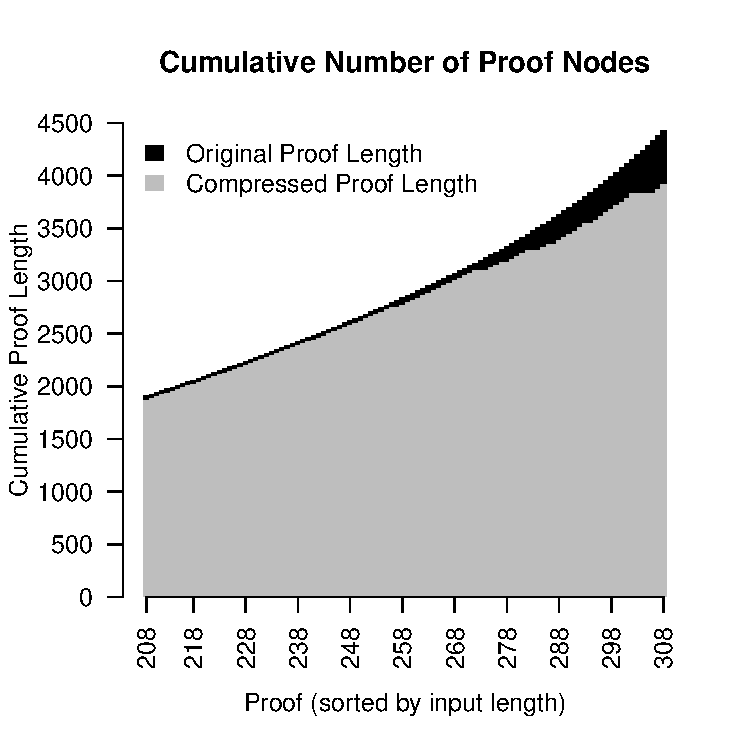
\includegraphics[scale=0.5]{images/cumulative_res_nodes_no_subs_top100.pdf}
%\end{figure}




% \begin{figure}
% 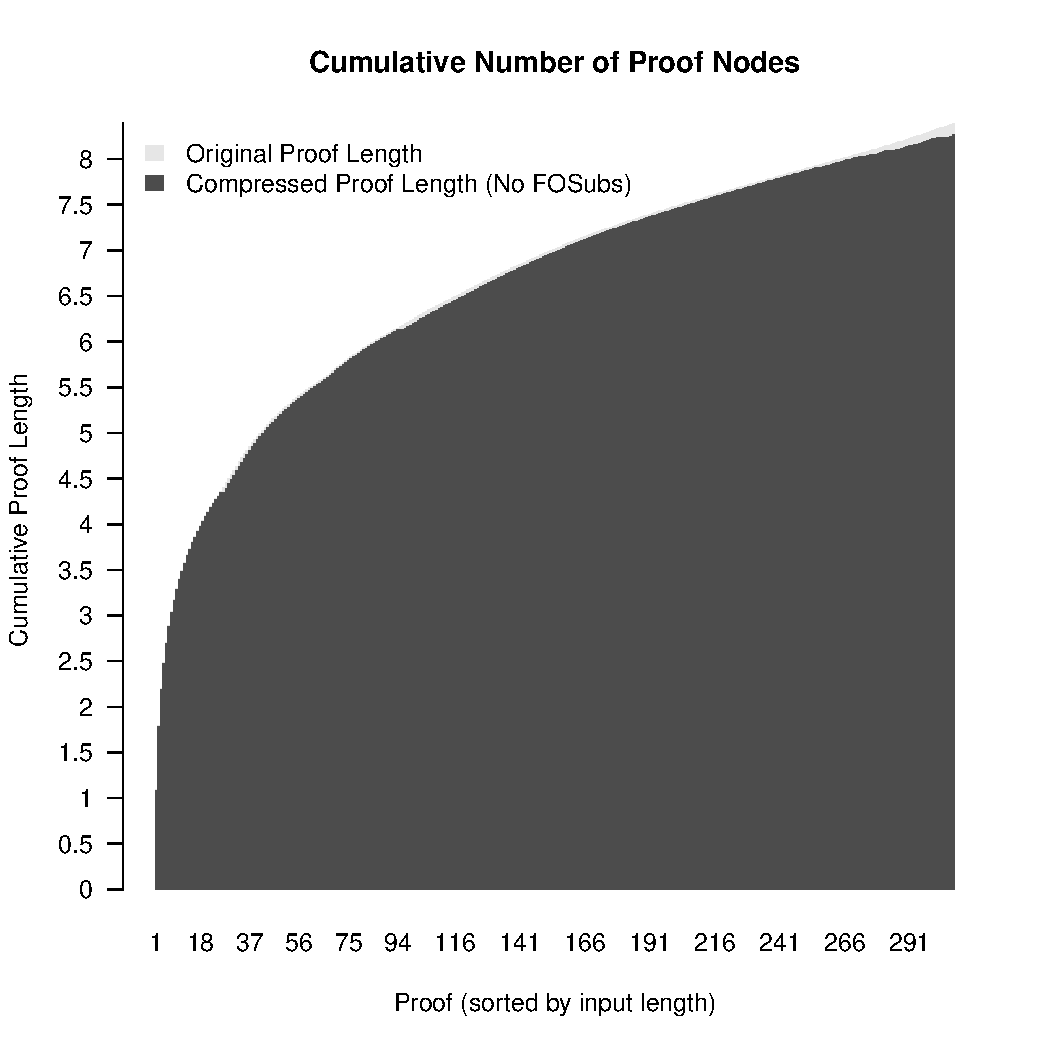
\includegraphics[scale=0.5]{images/cumulative_res_nodes_no_subs_log.pdf}
% \end{figure}
% \begin{figure}
% 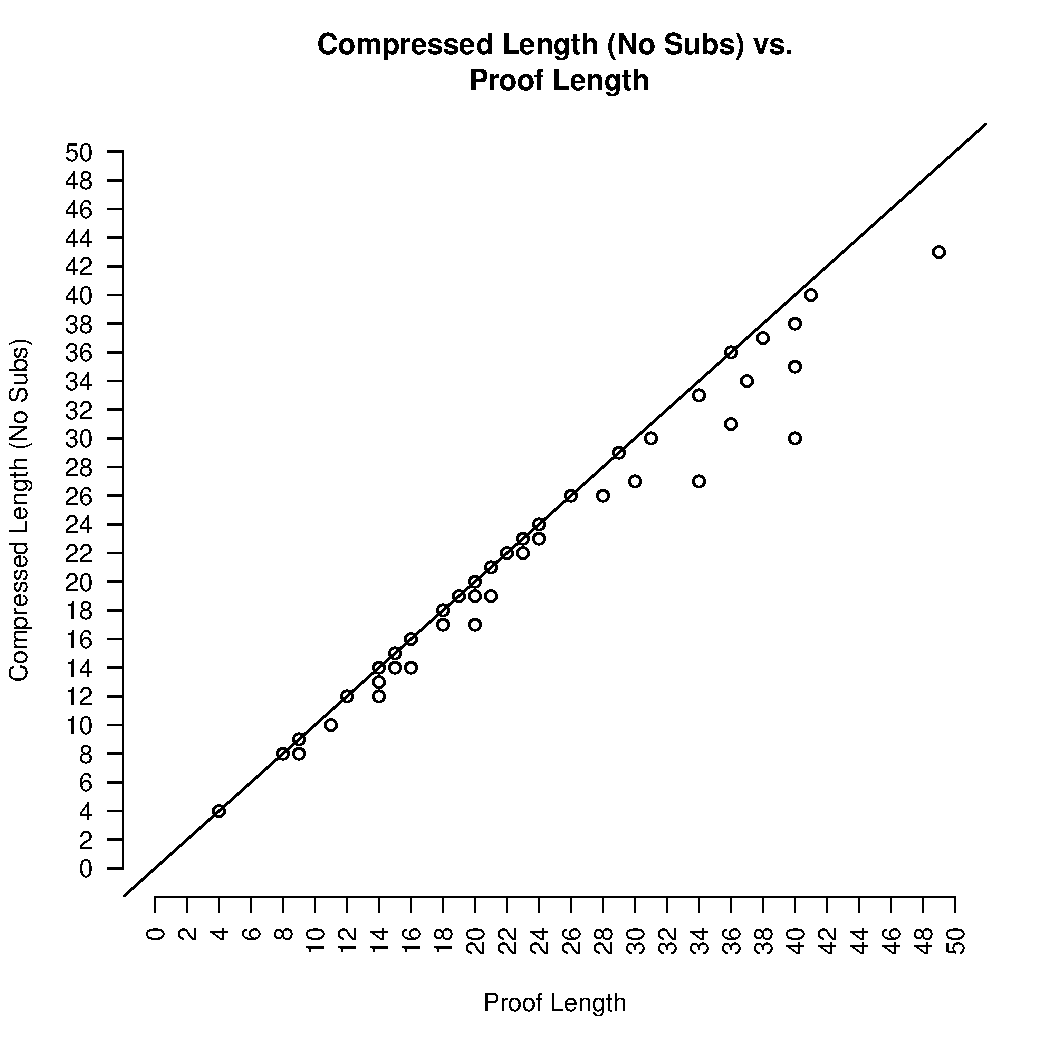
\includegraphics[scale=0.5]{images/compress_length_no_sub_vs_length.pdf}
% \end{figure}

%\begin{figure}%USED
%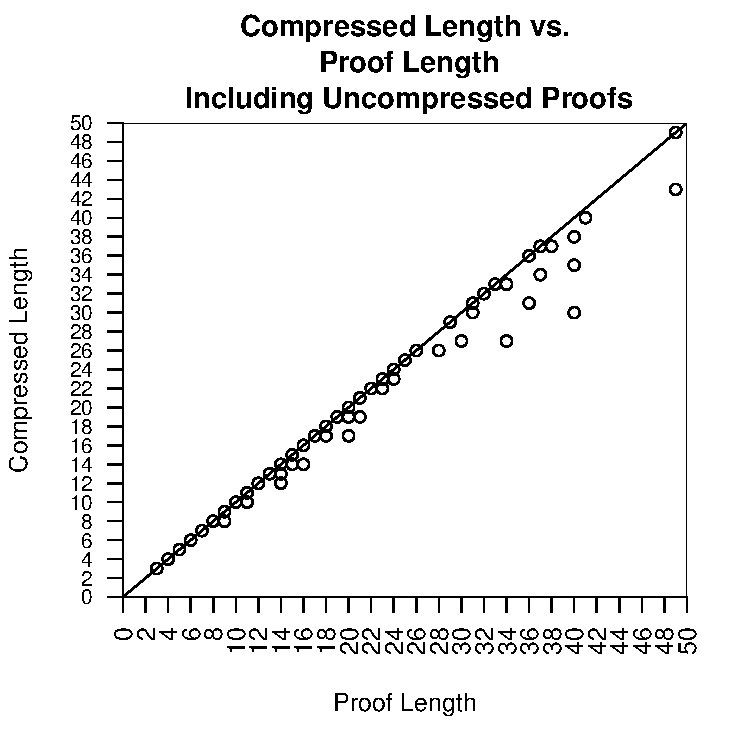
\includegraphics[scale=0.5]{images/compress_length_no_sub_vs_length_all_proofs.pdf}
%\end{figure}